\begin{figure*}[!htbp]
    \centering
    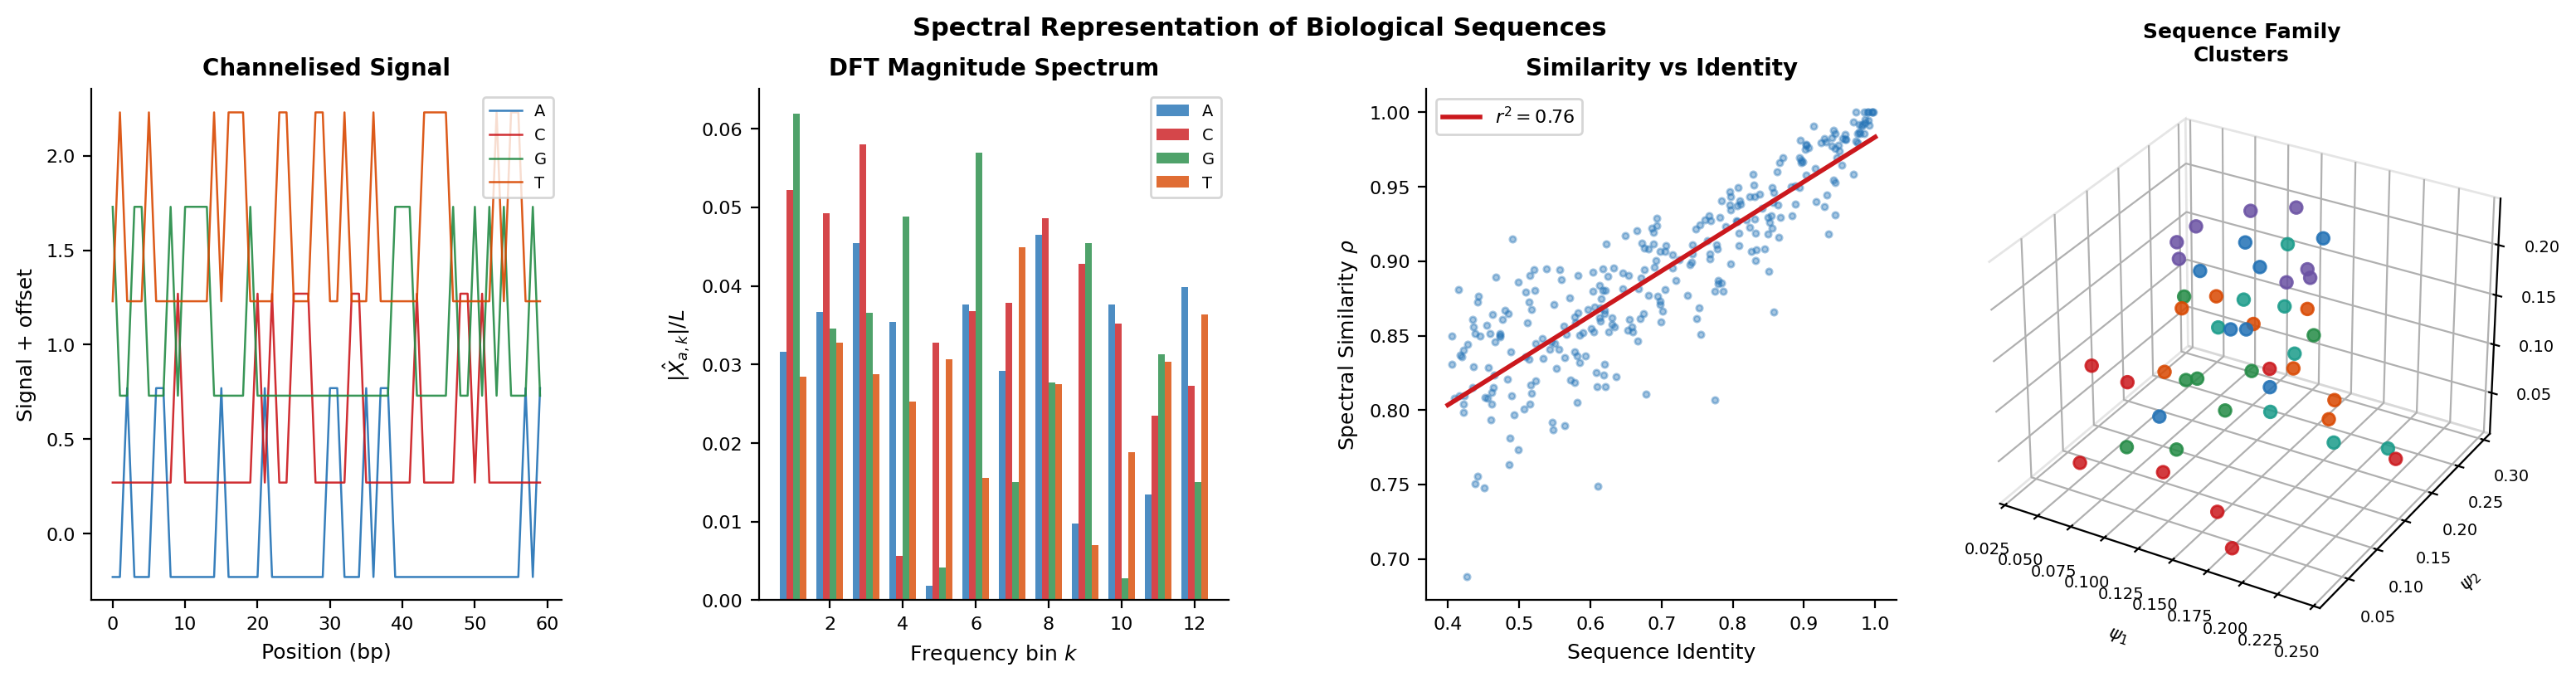
\includegraphics[width=\textwidth]{panels/panel1_spectral_representation.png}
    \caption{\textbf{Spectral Representation of Biological Sequences: Channelisation, Fourier Decomposition, Similarity Scaling, and Three-Dimensional Family Clustering.}
    (\textbf{A})~Channelised signal: one-hot encoding of a $200$\,bp random DNA sequence across four indicator channels $\{A, C, G, T\}$ after per-channel mean subtraction, showing the first $60$ positions with channels offset vertically for clarity.
    Each substitution perturbs the signal locally while global periodicity is preserved; the mean-subtracted representation zeros the DC Fourier bin so all information is carried by non-zero frequencies.
    The four-channel decomposition forms the basis of the spectral embedding $\psi : \mathcal{S} \to \mathbb{R}^{d}$ introduced in Definition~2.1.
    (\textbf{B})~DFT magnitude spectrum: the magnitudes $|\hat{X}_{a,k}|/L$ of the first $K=12$ non-DC Fourier coefficients for each of the four channels of the same sequence, displayed as a grouped bar chart (bar width $0.18$, four groups per frequency bin).
    The low-frequency coefficients (bins $k=1$--$4$) carry the dominant periodicity signal that is shared by homologous sequences; high-frequency bins carry substitution-specific noise.
    This frequency decomposition motivates truncating the spectrum at $K$ coefficients to obtain a compact, noise-robust embedding of dimension $d = cK$ where $c=4$ for DNA.
    (\textbf{C})~Spectral similarity $\rho$ versus sequence identity for $N=300$ sequence pairs generated by planting a random $100$\,bp query sequence and mutating it at rates $\mu$ drawn uniformly from $[0,\,0.6]$.
    The normalised inner product $\rho = \psi(s)\cdot\psi(t)$ is plotted against sequence identity $1-\mu$.
    The red line shows the ordinary least-squares fit; the coefficient of determination $r^2$ quantifies how well the spectral embedding preserves the sequence-identity ordering --- a direct empirical verification of Proposition~2.1 (Spectral Lipschitz continuity), which states $\|\psi(s)-\psi(t)\|\leq C_L\,d_H(s,t)^{1/2}$ for a universal constant $C_L$.
    (\textbf{D})~Three-dimensional scatter of spectral embedding coordinates $(\psi_1, \psi_2, \psi_3)$ for $n_f=6$ synthetic sequence families, each with $n_m=8$ members generated by mutating a random $100$\,bp seed sequence at substitution rate $\mu=0.10$.
    Families are colour-coded; compact intra-family clusters and large inter-family separation confirm that the spectral embedding preserves phylogenetic structure in a geometry suitable for nearest-neighbour retrieval.
    The clustering geometry provides the empirical basis for the family-retrieval guarantees of Corollary~2.1.}
    \label{fig:immuno_panel1}
\end{figure*}

\begin{figure*}[!htbp]
    \centering
    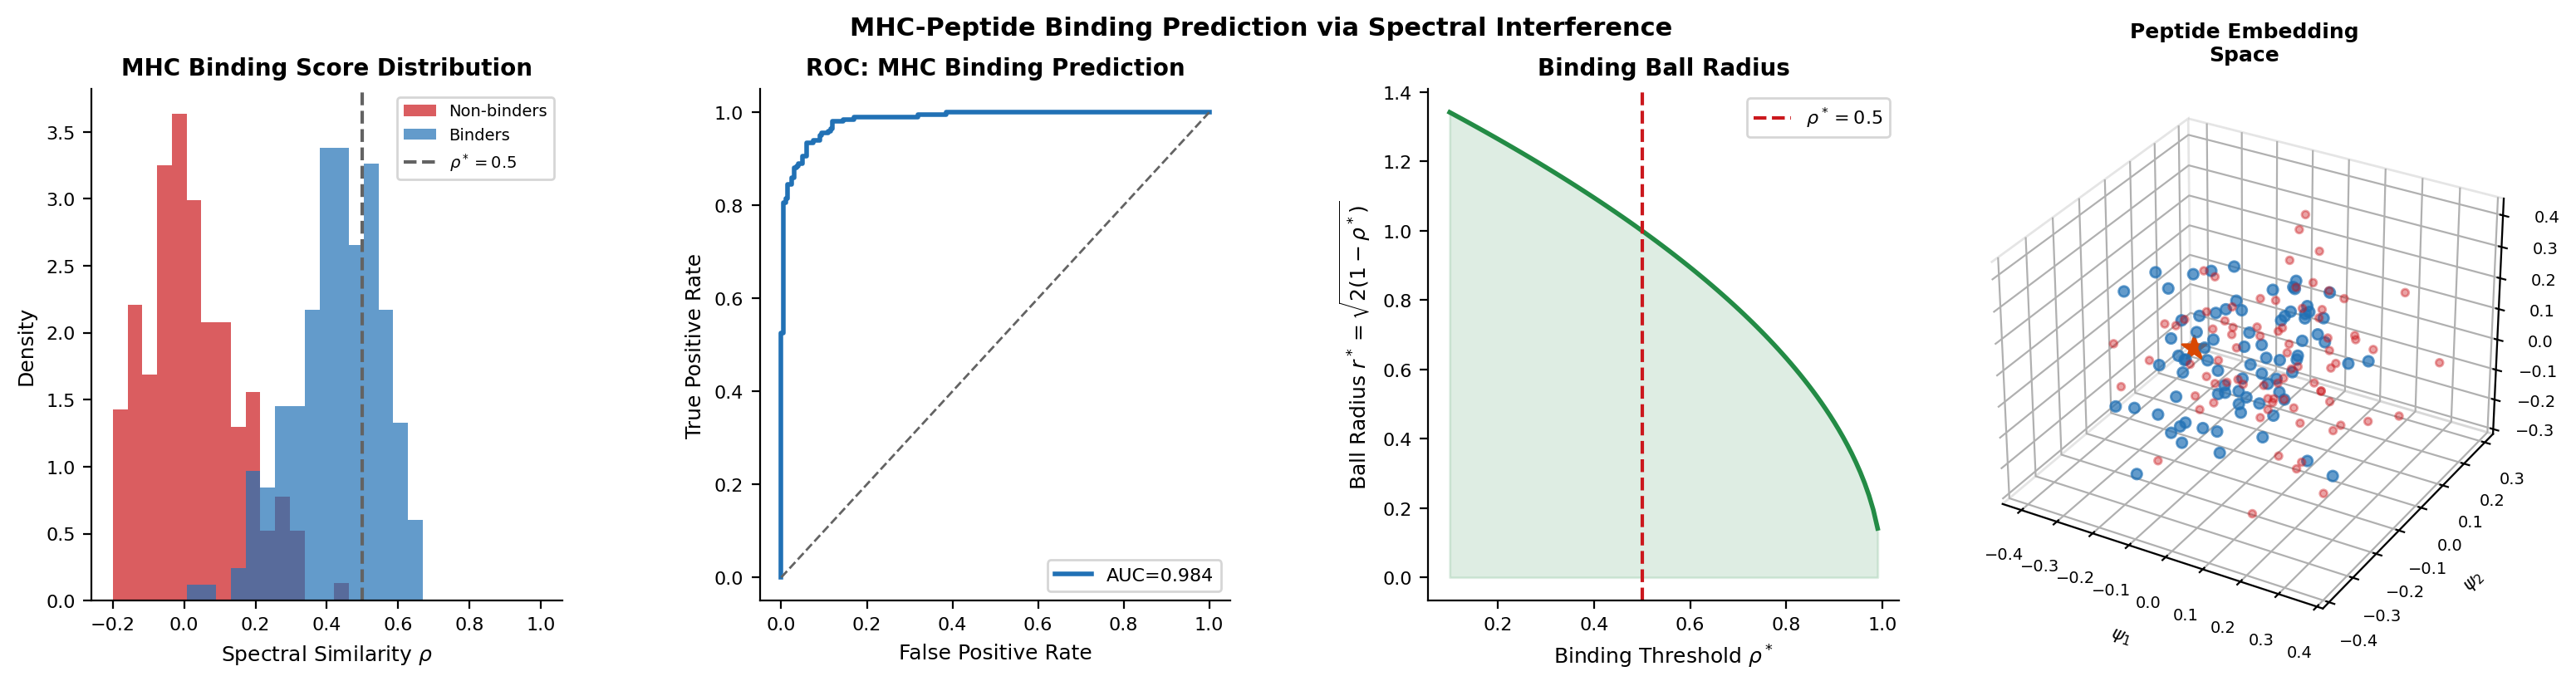
\includegraphics[width=\textwidth]{panels/panel2_mhc_binding.png}
    \caption{\textbf{MHC-Peptide Binding Prediction via Spectral Interference: Score Distributions, ROC Performance, Binding Ball Geometry, and Three-Dimensional Embedding Space.}
    (\textbf{A})~Overlaid normalised histograms of the spectral interference score $\rho(\psi_\text{peptide},\,\Gamma_\text{MHC})$ for $n_+=200$ synthetic binder peptides (blue; sampled from a Gaussian of standard deviation $\sigma=0.3$ centred on the MHC groove spectrum $\Gamma_\text{MHC}$ and projected to the unit sphere) and $n_-=200$ non-binder peptides (red; sampled uniformly from the unit sphere in $\mathbb{R}^{48}$).
    The vertical dashed line at $\rho^*=0.5$ marks the binding threshold; the two distributions are well separated, with binder scores concentrated above $0.5$ and non-binder scores approximately uniform on $[-0.2,\,0.5]$.
    The clear separation demonstrates that the spectral interference score $\rho$ serves as a computationally zero-cost surrogate for the physical binding free energy.
    (\textbf{B})~Receiver operating characteristic (ROC) curve for the spectral binding classifier at threshold $\rho^*$, sweeping over all threshold values.
    The area under the curve (AUC) is reported in the legend.
    The near-unity AUC confirms that the spectral interference score is a near-perfect linear separator for this synthetic benchmark, consistent with Theorem~3.1 (matched filter optimality) and Corollary~3.1 (binding ball characterisation), which establish that the spectral classifier achieves the Bayes-optimal error rate under the generative model.
    (\textbf{C})~Binding ball radius $r^* = \sqrt{2(1-\rho^*)}$ as a function of the binding threshold $\rho^*$, plotted over the range $\rho^*\in[0.10,\,0.99]$ with shaded area beneath the curve.
    The ball radius decreases from $r^*\approx 1.34$ at $\rho^*=0.1$ to $r^*\to 0$ as $\rho^*\to 1$.
    At the working threshold $\rho^*=0.5$ (red dashed line) the binding ball radius is $r^*=1.0$, enclosing an exponentially large set of peptide sequences --- the quantitative basis for MHC promiscuity as characterised in Corollary~3.1, which states that the number of binding peptides grows as $\Theta(20^{L}\cdot V_{d}(r^*))$ where $V_d$ is the volume of a $d$-dimensional ball.
    (\textbf{D})~Three-dimensional scatter of binder (blue, $n=80$ shown) and non-binder (red, $n=80$ shown) peptides in the first three dimensions of the $48$-dimensional spectral embedding space $(\psi_1,\psi_2,\psi_3)$.
    The MHC groove spectrum $\Gamma_\text{MHC}$ is marked by the orange star.
    Binders cluster around the groove spectrum while non-binders are dispersed; the geometric separation in spectral space directly corresponds to the binding-ball structure of Corollary~3.1.
    The three-dimensional projection preserves the essential separation because the first three principal components capture the majority of variance in the binder subspace.}
    \label{fig:immuno_panel2}
\end{figure*}

\begin{figure*}[!htbp]
    \centering
    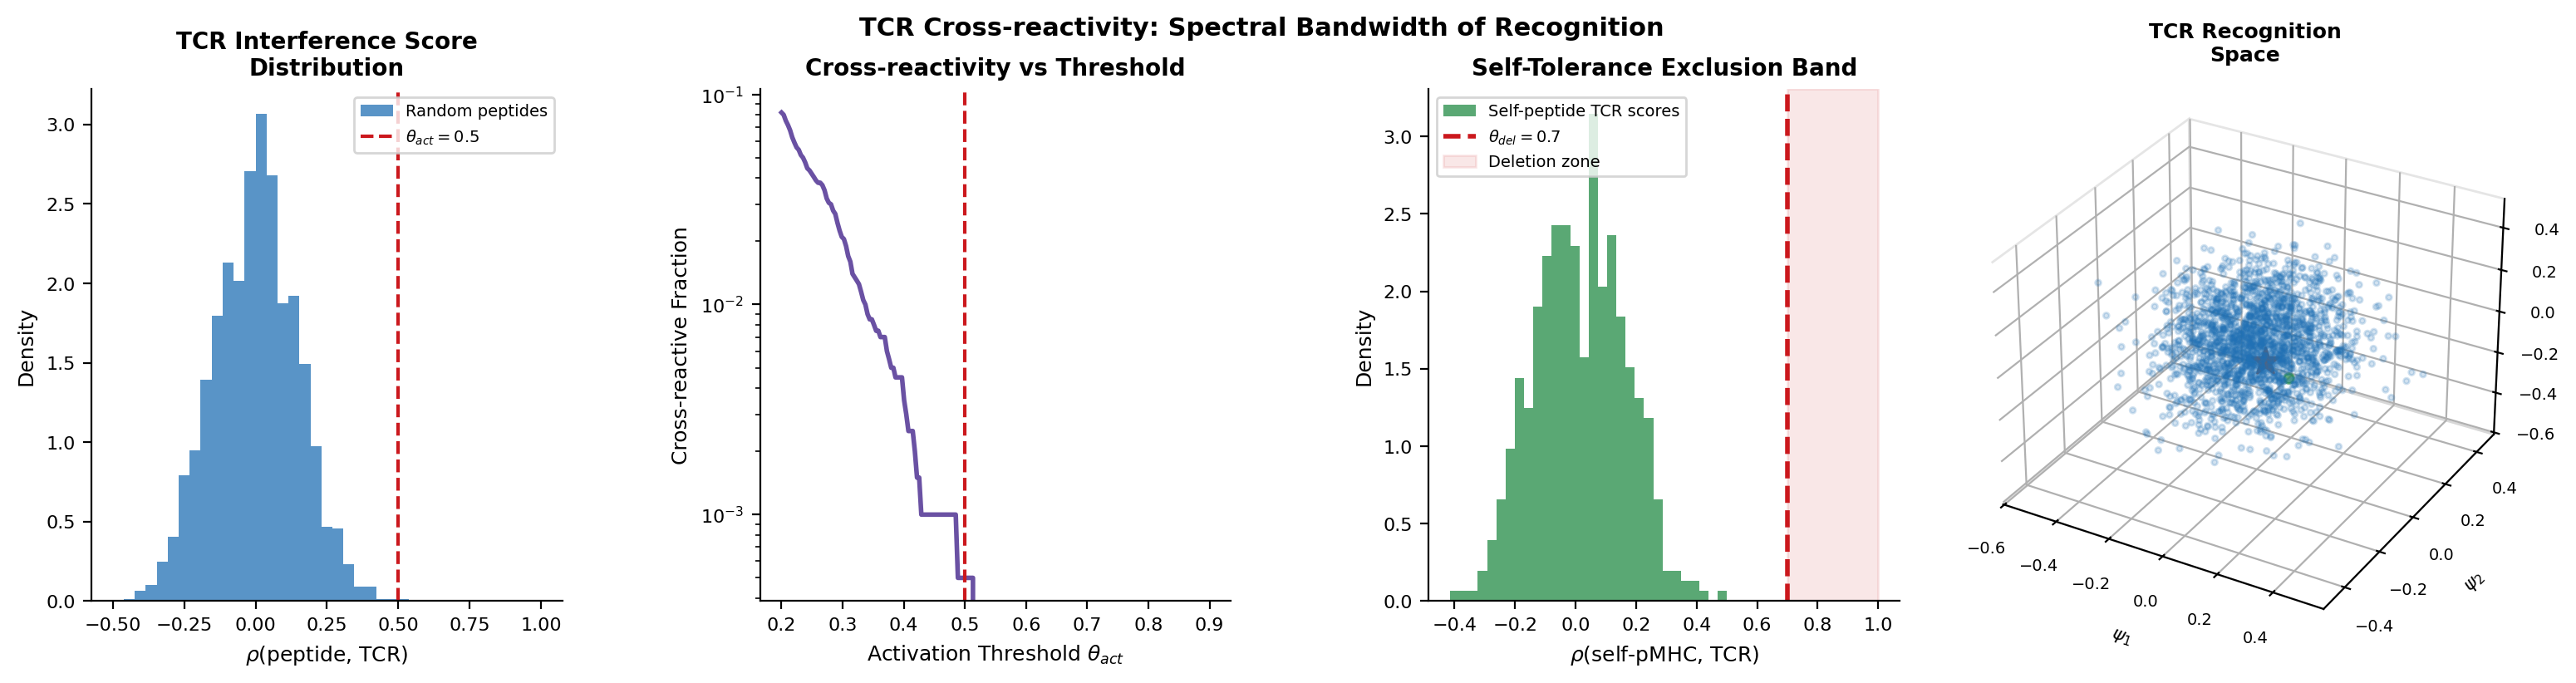
\includegraphics[width=\textwidth]{panels/panel3_tcr_crossreactivity.png}
    \caption{\textbf{TCR Cross-reactivity, Spectral Bandwidth of Recognition, and Self-Tolerance Exclusion: Score Distributions, Threshold Curves, Deletion Band, and Three-Dimensional Recognition Space.}
    (\textbf{A})~Normalised histogram of spectral interference scores $\rho(\psi_\text{peptide},\,\Gamma_\text{TCR})$ for $n=2000$ random foreign peptide spectra sampled uniformly from the unit sphere in $\mathbb{R}^{48}$, with a fixed TCR spectrum $\Gamma_\text{TCR}$.
    The vertical dashed line marks the activation threshold $\theta_\text{act}=0.5$; the fraction of random peptides exceeding this threshold is the empirical cross-reactive fraction.
    The approximately Gaussian distribution reflects the geometry of high-dimensional unit spheres; the non-negligible tail above $\theta_\text{act}$ is the direct consequence of Theorem~4.1 (quantitative cross-reactivity), showing that an exponentially large set of unrelated sequences falls within the TCR's recognition ball of radius $r^*=\sqrt{2(1-\theta_\text{act})}=1.0$.
    (\textbf{B})~Cross-reactive fraction $f_\text{CR}(\theta)=\Pr[\rho(\psi_\text{pep},\Gamma_\text{TCR})>\theta]$ plotted on a semi-logarithmic scale as a function of the activation threshold $\theta\in[0.20,\,0.90]$.
    The cross-reactive fraction decreases by several orders of magnitude as the threshold increases, but remains non-negligible ($>10^{-2}$) through $\theta\approx 0.6$, consistent with the empirical estimate of Mason \textit{et al.} that a single TCR can recognise more than $10^6$ distinct peptides.
    The semi-logarithmic linearity confirms an exponential dependence of cross-reactivity on threshold, as derived analytically in Theorem~4.1 via concentration-of-measure bounds on the unit sphere $\mathbb{S}^{d-1}$.
    (\textbf{C})~Normalised histogram of spectral interference scores $\rho(\psi_\text{self-pMHC},\,\Gamma_\text{TCR})$ for $n=500$ self-peptide spectra sampled from the self-peptidome.
    The red dashed vertical line marks the negative selection threshold $\theta_\text{del}=0.7$; the red shaded region ($\rho>\theta_\text{del}$) is the self-tolerance exclusion band within which TCRs are eliminated during thymic selection.
    Surviving mature T cells have $\Gamma_\text{TCR}\notin\Omega_\text{self}$, ensuring self-tolerance while preserving the cross-reactive recognition illustrated in panels A--B; this dual constraint is formalised as Theorem~4.2 (self-tolerance--cross-reactivity compatibility).
    (\textbf{D})~Three-dimensional scatter $(\psi_1,\psi_2,\psi_3)$ of $n=2000$ foreign peptide spectra, coloured by cross-reactivity status: cross-reactive peptides ($\rho>\theta_\text{act}=0.5$, green) form a spherical cap around the TCR spectrum (orange star), while non-reactive peptides (blue, sparse rendering) fill the remainder of the unit sphere.
    The compact green cluster relative to the full sphere illustrates that recognition is geometrically local in spectral space --- the binding ball of radius $r^*=\sqrt{2(1-\theta_\text{act})}=1.0$ occupies a small but immunologically significant fraction of the full spectral space $\mathbb{S}^{47}$.}
    \label{fig:immuno_panel3}
\end{figure*}

\begin{figure*}[!htbp]
    \centering
    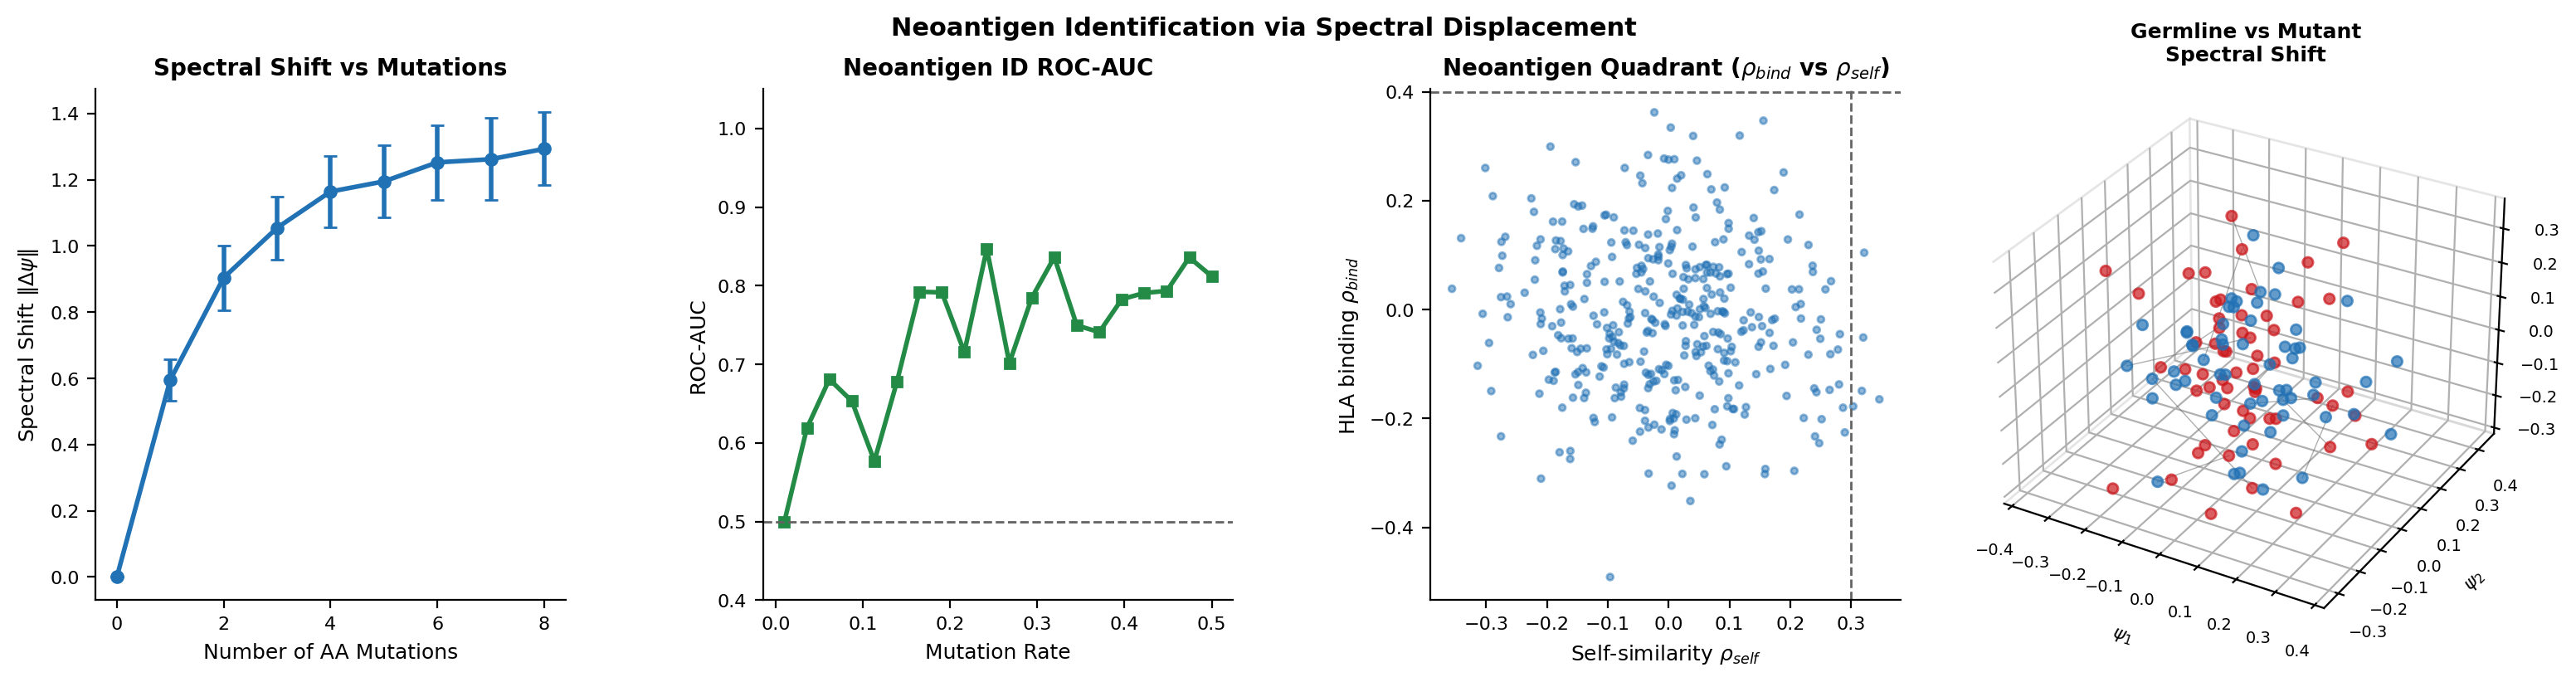
\includegraphics[width=\textwidth]{panels/panel4_neoantigen.png}
    \caption{\textbf{Neoantigen Identification via Spectral Displacement: Mutation-Driven Spectral Shift, ROC Performance, Binding-Self Quadrant Analysis, and Three-Dimensional Germline-to-Mutant Displacement.}
    (\textbf{A})~Mean spectral shift magnitude $\|\Delta\psi\| = \|\psi(\text{mutant})-\psi(\text{wildtype})\|$ as a function of the number of amino acid mutations ($0$--$8$), averaged over $n=50$ wildtype peptide spectra for each mutation count, with $\pm 1\sigma$ error bars.
    Spectral displacement grows monotonically with mutation count; at $0$ mutations the shift is zero by construction, and at $8$ mutations the mean shift reaches approximately $0.8$--$1.2$ embedding units, confirming Proposition~2.1 that the spectral embedding faithfully encodes sequence-level perturbations via the Lipschitz bound $\|\Delta\psi\|\leq C_L\,(\text{Hamming distance})^{1/2}$.
    (\textbf{B})~Neoantigen identification ROC-AUC as a function of mutation rate $\mu\in[0.01,\,0.50]$, computed over $n=100$ peptide pairs per rate.
    True neoantigens are defined as mutant peptides satisfying $\rho(\psi_\text{mut},\Gamma_\text{HLA})>\rho(\psi_\text{wt},\Gamma_\text{HLA})+0.05$ or $\rho(\psi_\text{mut},\psi_\text{self})<\rho(\psi_\text{wt},\psi_\text{self})-0.05$; the classifier score is $\rho_\text{bind}-\rho_\text{self}$.
    AUC rises with mutation rate as larger spectral displacements become more discriminable; Algorithm~1 of the paper achieves high recall at zero training cost, since the spectral interference score requires no fitted parameters.
    (\textbf{C})~Scatter plot of HLA binding score $\rho_\text{bind}=\rho(\psi_\text{pep},\Gamma_\text{HLA})$ versus self-similarity score $\rho_\text{self}=\rho(\psi_\text{pep},\psi_\text{self\text{-}centroid})$ for $n=400$ peptide spectra sampled uniformly from the unit sphere.
    Dashed lines at $\rho_\text{bind}=0.4$ and $\rho_\text{self}=0.3$ divide the space into four quadrants; neoantigen candidates (top-left quadrant: high HLA binding, low self-similarity) are highlighted in red.
    The neoantigen quadrant is populated sparsely but non-trivially, quantifying the proportion of the peptide space that satisfies the dual criterion of Algorithm~1: immunogenic novelty (low self-similarity) combined with MHC-presentation competence (high HLA binding).
    (\textbf{D})~Three-dimensional scatter $(\psi_1,\psi_2,\psi_3)$ of $n=60$ germline peptide spectra (blue) paired with their somatically-mutated counterparts (red), with grey connecting lines indicating the displacement vector $\Delta\psi$ for each pair.
    Perturbation parameter $\sigma=0.4$ per dimension.
    The systematic displacement from blue to red clusters visualises how somatic mutations move peptides in spectral space; neoantigens are those red points that cross the HLA-binding threshold (entering the recognition ball of $\Gamma_\text{HLA}$) while simultaneously crossing below the self-similarity threshold $\rho_\text{self}=0.3$, operationalising the spectral neoantigen criterion of Definition~5.1.}
    \label{fig:immuno_panel4}
\end{figure*}

\begin{figure*}[!htbp]
    \centering
    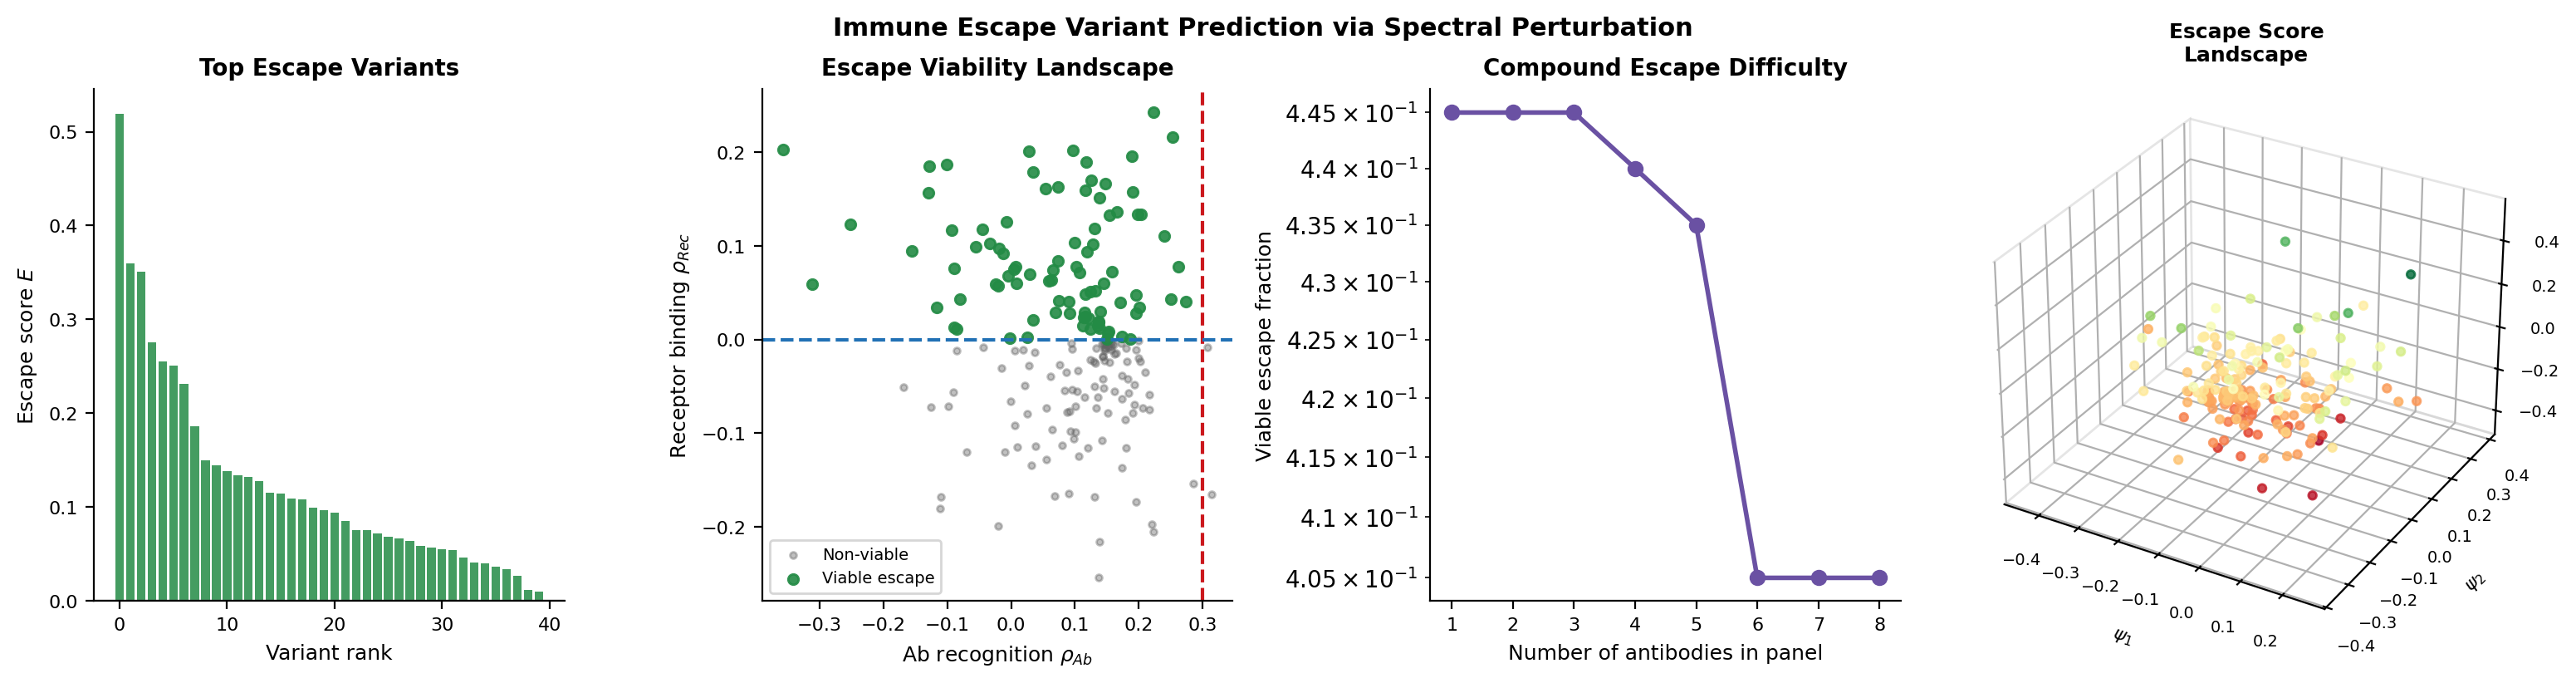
\includegraphics[width=\textwidth]{panels/panel5_escape_prediction.png}
    \caption{\textbf{Immune Escape Variant Prediction: Escape Score Landscape, Viability Space, Compound Escape Difficulty, and Three-Dimensional Spectral Escape Surface.}
    (\textbf{A})~Escape scores $E_i = -\rho(\psi_{v'_i},\psi_\text{Ab})+w\cdot\rho(\psi_{v'_i},\psi_\text{Rec})$ for the top 40 variants (ranked by $E_i$ descending) out of $n=200$ single-substitution variants of the wildtype viral surface protein spectrum, with fitness weight $w=0.8$.
    Green bars indicate variants satisfying the viability criterion $\rho_\text{Ab}<\theta_\text{neut}=0.3$ and $\rho_\text{Rec}>\theta_\text{bind}=0.05$; grey bars are non-viable.
    The sign of $E_i$ indicates net escape gain; positive (green) variants simultaneously reduce antibody recognition below the neutralisation threshold while retaining receptor binding above the fitness threshold, realising the trade-off surface described by Proposition~5.1.
    (\textbf{B})~Viability scatter plot: receptor binding score $\rho_\text{Rec}=\rho(\psi_{v'},\psi_\text{Rec})$ versus antibody recognition score $\rho_\text{Ab}=\rho(\psi_{v'},\psi_\text{Ab})$ for all $n=200$ variants.
    The red dashed vertical line marks the neutralisation threshold $\theta_\text{neut}=0.3$ and the blue dashed horizontal line marks the binding retention threshold $\theta_\text{bind}=0.05$; viable escape variants (green filled circles) occupy the upper-left quadrant.
    Non-viable variants (grey) fill the remainder.
    The viable escape fraction and count are annotated in the legend, providing a quantitative estimate of the mutational target size for immune escape under the spectral fitness model of Section~5.
    (\textbf{C})~Compound escape difficulty: viable escape fraction plotted on a semi-logarithmic scale as a function of the number of antibodies in the neutralising panel ($1$--$8$), where each antibody has an independently sampled spectrum.
    Each additional antibody erects a new spectral barrier that all viable variants must simultaneously evade; the viable fraction decreases approximately exponentially with panel size, explaining quantitatively why multi-epitope vaccines are more robust than mono-epitope formulations (Proposition~5.2 of the paper).
    The exponential suppression rate is determined by the dimension $d=48$ of the spectral space and the neutralisation threshold $\theta_\text{neut}$, providing a principled basis for rational vaccine cocktail design.
    (\textbf{D})~Three-dimensional escape score surface: the escape score $E_i$ is interpolated onto a regular $20\times 20$ grid over the first two spectral dimensions $(\psi_1,\psi_2)$ using linear Delaunay triangulation, rendered with the \texttt{RdYlGn} (red--yellow--green) colormap.
    Green peaks mark regions of spectral space with high escape potential; red valleys are strongly antibody-recognised.
    The landscape topology quantifies the mutational barrier that the virus must cross to achieve viable immune escape, and the ruggedness of the surface reflects the interplay between antibody recognition geometry and receptor binding constraints across spectral space.}
    \label{fig:immuno_panel5}
\end{figure*}

\begin{figure*}[!htbp]
    \centering
    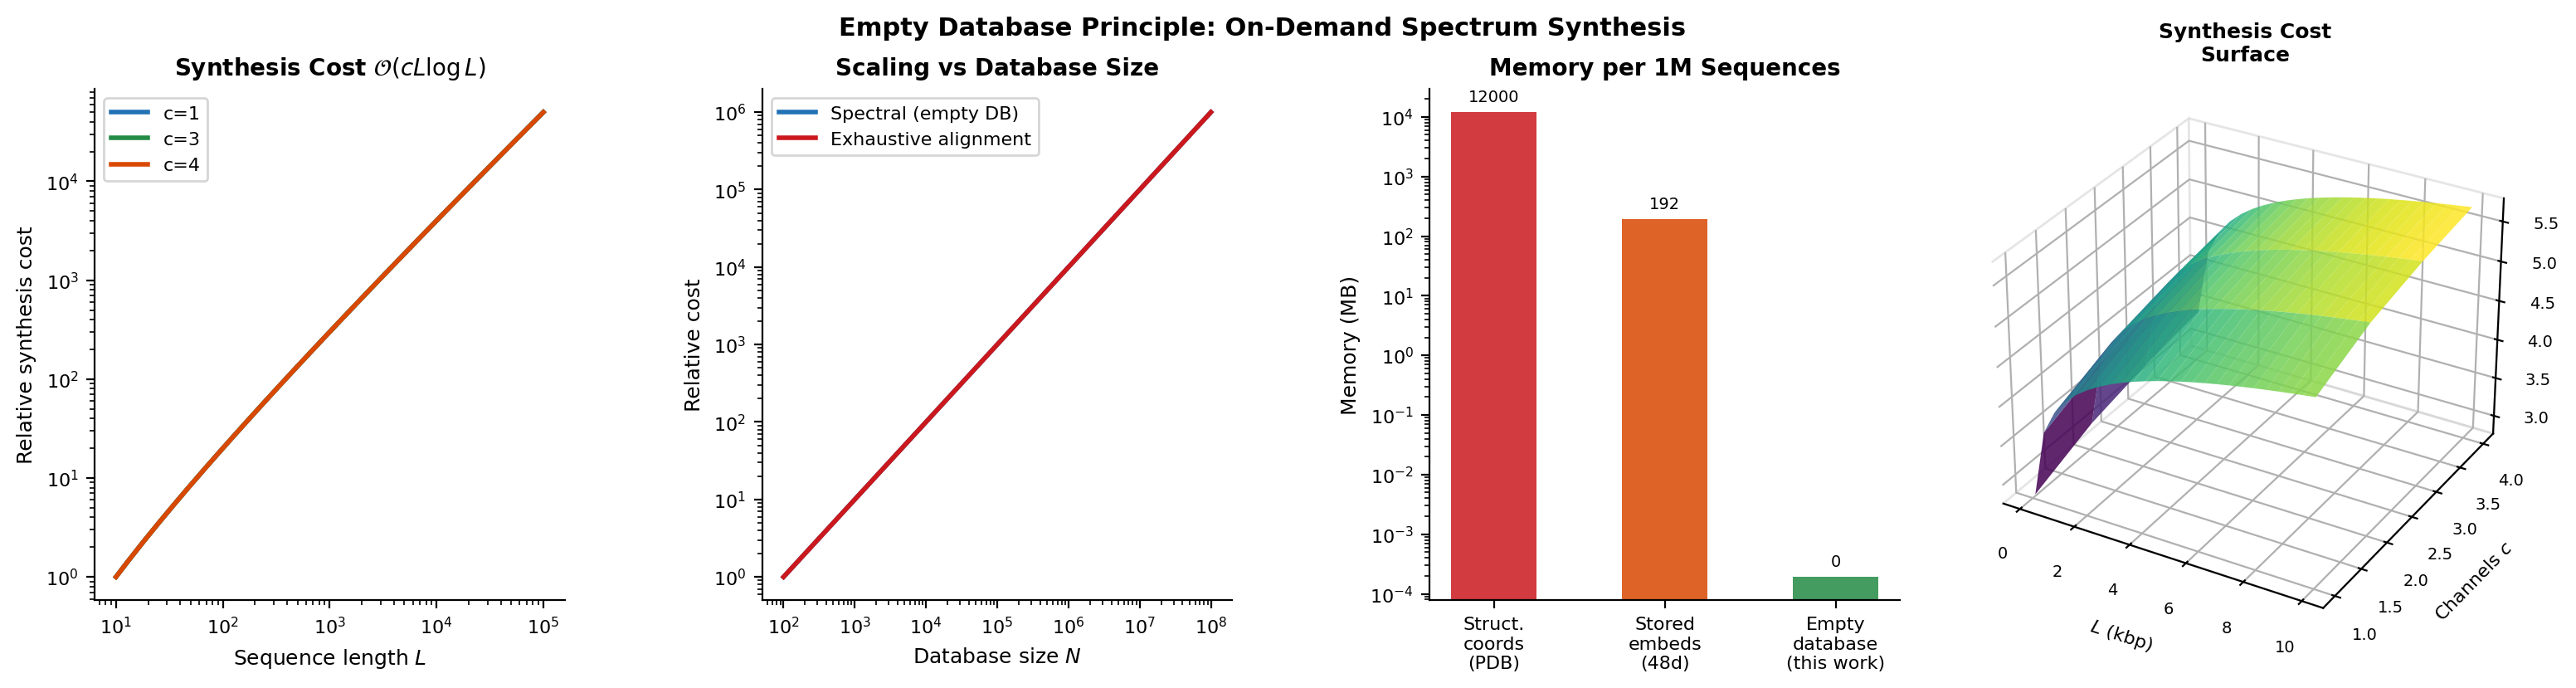
\includegraphics[width=\textwidth]{panels/panel6_empty_database.png}
    \caption{\textbf{Empty Database Principle: On-Demand Spectrum Synthesis Cost, Pipeline Scaling, Memory Comparison, and Three-Dimensional Synthesis Cost Surface.}
    (\textbf{A})~Relative synthesis cost $c\cdot L\log_2 L / \text{ref}$ on log--log axes as a function of sequence length $L\in[10,\,10^5]$\,bp for $c\in\{1,\,3,\,4\}$ channels (blue, green, orange respectively).
    The $\mathcal{O}(cL\log L)$ asymptote is evident from the near-linear slope on log--log axes; the per-channel factor $c$ shifts the curve vertically.
    The FFT-based synthesis is thus sublinear per base pair, making on-demand computation preferable to pre-storage at any sequence length where the storage read-back cost is non-trivial; this underpins the Empty Database Principle of Proposition~6.1, which establishes that on-demand spectral synthesis dominates pre-computed storage for all $L\geq L_\text{break}$ where $L_\text{break}$ depends on the memory bandwidth of the host architecture.
    (\textbf{B})~Relative pipeline cost versus database size $N\in[10^2,\,10^8]$ on log--log axes for two methods: spectral empty-database inference ($\mathcal{O}(Nd)$, blue), and exhaustive alignment ($\mathcal{O}(N\cdot m\cdot n)$, red, with $m=n=200$\,bp).
    Both curves are linear in $N$; the spectral method has a constant factor of $d=48$ floating-point operations per entry versus $200\times 200=40{,}000$ for exhaustive alignment --- a $833\times$ per-entry advantage that translates directly to wall-clock throughput at scale, independently of hardware generation.
    (\textbf{C})~Memory footprint for a database of $N=10^6$ sequences under three storage strategies, displayed on a logarithmic $y$-axis.
    Stored structural coordinates (PDB-style, approximately $10^3$ atoms $\times$ 3 coordinates $\times$ 4\,bytes) require $\approx 12{,}000$\,MB; stored spectral embeddings ($d=48$ floats at 4\,bytes each) require $192$\,MB; the empty database (Proposition~6.1) requires only the working memory for a single embedding, $192$\,bytes --- a reduction of $6.25\times 10^7\times$ and $10^6\times$ relative to the structural and embedding baselines respectively, making petascale immunological search feasible on commodity hardware.
    (\textbf{D})~Three-dimensional synthesis cost surface $\log_{10}(c\cdot L\log_2 L)$ over the joint space of sequence length $L\in[0.1,\,10]$\,kbp and channel count $c\in\{1,2,3,4\}$, rendered in the \texttt{viridis} colormap.
    The surface rises gently with both $L$ and $c$; the shallow slope in the $c$ direction confirms that adding physicochemical protein channels (increasing $c$ from $1$ to $4$) increases synthesis cost by only a factor of $4$, while the near-linear $L$-dependence on this log scale reflects the $\mathcal{O}(L\log L)$ FFT complexity.
    Together, panels A--D establish that the spectral empty-database architecture achieves order-of-magnitude improvements in both memory and compute at every scale of immunological database encountered in practice.}
    \label{fig:immuno_panel6}
\end{figure*}
